\documentclass[11pt,dvipdfmx]{jarticle}

\usepackage{eee}
\usepackage{subfig}
\usepackage{pdfpages}

\renewcommand{\labelenumi}{\alph{enumi}}
\renewcommand{\labelenumii}{\roman{enumii}}

\begin{document}
% トップページを書く
\begin{jikkenTitle}
	\gakunen{3} % 学年を記述。この行で全体の枠を表示
	\numTitle{4}{強磁性体のヒステリシス現象} % 実験番号、タイトルを記述
	\subTitle{} % サブタイトルがあれば記述
	\jikkenbi{令和4年5月12日(木)} % 実験日を記述
	\jikkenbiII{令和4年5月17日(木)} % 実験日を記述(二日目がある場合。ない場合はこの行をコメントアウト)
	\kyoudou{3325 谷下 文紀 3329 野島 奏一朗 3337吉野 曹生} % 共同実験者名を記述
	\kyoudouII{} % その他の共同実験者名を記述
	\yoteibi{/  }% 予定日を記述
	\yoteibiII{}% 予定日2を記述
	\yoteibiIII{}% 予定日3を記述
	\hanNumberName{4}{3333}{宮崎 永} % 班番号・学生番号・氏名を記述。この行でタイトルページの描画を終了
\end{jikkenTitle}

\section{目的}
本実験では
\begin{itemize}
	\item トランス鉄心に使用される強磁性体のB-H特性測定を通し磁気回路と磁性材料について理解する。
	\item 変圧器鉄心の交流化特性を測定し、測定原理と鉄心のヒステリシス損算出法を理解する。
	\item 変圧器における励磁電流、電力、位相差の変化を観測する。
\end{itemize}
ことを目的とする。

\section{原理}
\subsection{磁気回路}
\wfig{hys:jikikairo}に示すように断面積$S\,[\mathrm{m}^2]$、平均磁路長$L\,[\mathrm{m}]$の鉄心に巻数$N_1\,[\mathrm{Turn}]$のコイルを巻き、これに$I\,[\mathrm{A}]$の電流を流すと、起磁力$N_1\cdot I\,[\mathrm{A}\cdot\mathrm{Turn}]$を生じる。
この起磁力により
\begin{equation}
	\phi = \frac{N_1\cdot I}{R_m}
\end{equation}
の磁束$\phi\,[\mathrm{Wb}]$を生じる。ここで$R_m$は以下に示す磁気抵抗である。
\begin{equation}
	R_m= \frac{L}{\mu_0 \mu_s S}
\end{equation}
ただし、$\mu_0 = 4\pi\times 10^{-7}\,\mathrm{F/m}$ は真空の透磁率であり、$\mu_s$は鉄心の比透磁率である。
ここで、磁路1\,mあたりの起磁力を磁化力$H\,[\mathrm{A/m}]$という。 磁化力$H$は
\begin{equation}
	H=\frac{N_1\cdot I}{L}
\end{equation}
である。また磁路断面積 1\,m$^2$あたりの磁束を、磁束密度$B\,[\mathrm{Wb/m}^2]$という。
\begin{equation}
	B=\frac{\phi}{S}
	\label{eq:hys:BphiS}
\end{equation}
ここで、$S\,[\mathrm{m}^2]$は磁路断面積を示す。
\begin{figure}[htbp]
	\centering
	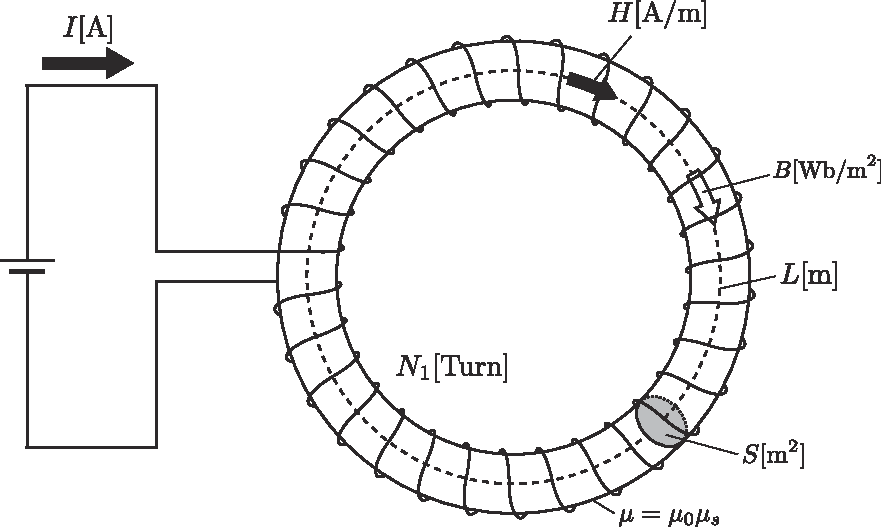
\includegraphics[width=70mm]{fig/magnetism_circuit.pdf}
	\caption{磁気回路}
	\label{fig:hys:jikikairo}
\end{figure}

鉄心の磁化力$H$と磁束密度$B$との関係を示す曲線をB-H曲線といい、一般に\wfig{hys:bhcurve}(a)のような飽和特性になる。
また磁化力$H$を正負の方向に増減すると、\wfig{hys:bhcurve}(b)の様なヒステリシス曲線になる。
\begin{figure}[htbp]
	\centering
	\begin{tabular}{cc}
		\includegraphics[width=70mm]{fig/bhcurve.pdf} &
		\includegraphics[width=70mm]{fig/hysteresis.pdf}             \\
		(a) B-H 曲線                                    & (b) ヒステリシス曲線
	\end{tabular}
	\caption{B-H曲線とヒステリシス曲線}
	\label{fig:hys:bhcurve}
\end{figure}

\subsection{交流磁化特性}
\wfig{hys:transformer}の変圧器のように、鉄心に巻かれた巻数$N_1$のコイルに交流電圧$V_1$を加えると、鉄心中に交番磁束$\phi$を作るための電流(励磁電流)$i_0$が流れる。このとき磁束密度$B$と磁化力$H$との間にはヒステリシス特性があるため、励磁電流は\wfig{hys:hizumi}のようにひずみを生ずる。この現象を逆に利用して、励磁電流$i_0$と交番磁束$\phi$の波形をなんらかの方法で取り出し、オシロスコープのX軸に励磁電流$i_0$の波形、Y軸に交番磁束$\phi$の波形を入力すれば、オシロスコープの画面に鉄心のヒステリシス特性(B-H曲線)が描かれる。
\begin{figure}[htbp]
	\centering
	\includegraphics[width=140mm]{fig/transformer.pdf}
	\caption{変圧器の交流磁化特性測定回路}
	\label{fig:hys:transformer}
\end{figure}

励磁電流$i_0$の波形を直接取り出すのは難しいので、\wfig{hys:transformer}において励磁電流$i_0$が抵抗$R_h$を流れるときの電圧変化、すなわち
\begin{equation}
	V_h = i_0R_h
\end{equation}
として取り出す。また、交番磁束$\phi$は次の様にして取り出す。

\wfig{hys:transformer}において二次巻線$N_2$と鎖交する磁束の時間に対する変化が二次誘起電圧$e_2$として現れるから
\begin{equation}
	e_2 = -N_2\frac{d \phi}{dt}
	\label{eq:hys:e2}
\end{equation}
となり、\weq{hys:e2}を変形すると
\begin{equation}
	d \phi = \frac{1}{N_2}\times e_2\times dt
	\label{eq:hys:dphi}
\end{equation}
となるから、交番磁束$\phi$は\weq{hys:dphi}を積分すれば求まることとなる。すなわち、二次巻線に発生する電圧$e_2$を時間で積分すればよい。そこで二次側にCR積分回路を接続しコンデンサCの両端から$e_2$を積分した、交番磁束に比例した電圧をとりだす。

\begin{figure}[htb]
	%\begin{center}
	\centering
	\subfloat[ヒステリシス現象のない場合]{
		\includegraphics[width=115mm]{fig/hizumi_a.pdf}
	}
	\vspace{5mm}
	\subfloat[ヒステリシス現象のある場合]{
		\includegraphics[width=115mm]{fig/hizumi_b.pdf}
	}
	\caption{ヒステリシス現象}
	\label{fig:hys:hizumi}
	%\end{center}    
\end{figure}

\section{方法}
\subsection{使用器具}
今回の実験で使用した器具を表\ref{tab:使用器具}に示す。
また、これらの器具を用いてのように配線を行った回路を図\ref{fig:circuit}と図\ref{fig:circuit_int}に示す。
\begin{table}[htbp]
	\centering
	\caption{使用器具}
	\begin{tabular}{lll}
		使用器具            & 製造元      & 型番          \\ \hline \hline
		電圧計             & YEW      & TYPE2013    \\ \hline
		電流計             & YOKOGAWA & TYPE2013    \\ \hline
		電力計             & YOKOGAWA & MODEL 2041  \\ \hline
		スライダートランス       & 東京理工舎    & RSA-2       \\ \hline
		オシロスコープ         & KEYSIGHT & MSO-X 2004A \\ \hline
		ヒステリシス曲線直視回路セット & 不明       & 不明          \\ \hline
	\end{tabular}
	\label{tab:使用器具}
\end{table}

\begin{figure}[htbp]
	\centering
	\includegraphics[keepaspectratio, scale=0.6]{circuit.pdf}
	\caption{実験回路(積分回路なし)}
	\label{fig:circuit}
\end{figure}
\begin{figure}[htbp]
	\centering
	\includegraphics[keepaspectratio, scale=0.5]{circuit_int.pdf}
	\caption{実験回路(積分回路あり)}
	\label{fig:circuit_int}
\end{figure}

\subsection{実験手順}
本実験では、励磁電流及び電力、位相差の測及び交流磁化特性の測定を行った。次にそれぞれの実験手順を示す。
\subsubsection{励磁電流及び電力、位相差の測定}
\begin{enumerate}[1)]
	\item 図\ref{fig:circuit}に示した回路のように、各種計器とスライダック、ヒステリシス曲線直視回路セットオ及びトランスを接続した。
	\item スライダックの電圧を0Vに設定し、オシロスコープのプローブを次のように接続した。
	      \begin{itemize}
		      \item CH1のプローブのGNDを図\ref{fig:circuit}のC点
		      \item CH1のプローブの先端を図\ref{fig:circuit}のA点
		      \item CH2のプローブのGNDを図\ref{fig:circuit}のC点
		      \item CH2のプローブの先端を図\ref{fig:circuit}のB点
	      \end{itemize}
	\item オシロスコープの水平感度を$5\, \mathrm{ms/DIV}$に設定した。
	\item オシロスコープのCH1の垂直感度を$50\,\mathrm{V/DIV}$、CH2の垂直感度を$500\,\mathrm{mV/DIV}$に設定した。
	\item オシロスコープのCH2は反転モードに設定した。
	\item 入力電圧を75Vから100Vまで5V刻みで変化させ、それぞれ電流と有効電力を測定した。
	\item 入力電圧が80Vと100Vの時はオシロスコープで波形を観測し、USBに保存した。オシロスコープのCH2は反転モードに設定した。
\end{enumerate}

\subsubsection{交流磁化特性の測定}
\begin{enumerate}[1)]
	\item 図\ref{fig:circuit_int}に示した回路のように、各種計器とスライダック、ヒステリシス曲線直視回路セット及びトランスを接続した。
	\item	スライダックの電圧を0Vに設定し、オシロスコープのプローブをそれぞれ次のように接続した。
	      \begin{itemize}
		      \item CH1のプローブのGNDを図\ref{fig:circuit_int}のC点
		      \item CH1のプローブの先端を図\ref{fig:circuit_int}のB点
		      \item CH2のプローブのGNDを図\ref{fig:circuit_int}のE点
		      \item CH2のプローブの先端を図\ref{fig:circuit_int}のD点
	      \end{itemize}
	\item オシロスコープのCH1の垂直感度を$500\, \mathrm{mV/DIV}$、CH2を$20\, \mathrm{mV/DIV}$に設定した。
	\item オシロスコープの水平感度表示をX-Y表示に変更した。
	\item	入力電圧を80Vと100Vに設定し、それぞれオシロスコープで波形を観測し、USBに保存した。
\end{enumerate}
\newpage

\section{結果}
\subsection{励磁電流及び電力、位相差の測定結果}
\begin{table}[htbp]
	\centering
	\caption{励磁電流及び電力の測定結果}
	\begin{tabular}{llll}
		電圧$v\,[\mathrm{V}$] & 電流$i_0\,[\mathrm{A}]$ & 電力$P_0\,[\mathrm{W}]$ & 位相差$\theta \,[\mathrm{deg}]$ \\ \hline	\hline
		75                  & 41.0                  & 0.9                   & 73.0                         \\ \hline
		80                  & 45.0                  & 1                     & 73.9                         \\	\hline
		85                  & 49.5                  & 1.1                   & 74.8                         \\	\hline
		90                  & 54.5                  & 1.3                   & 74.6                         \\	\hline
		95                  & 60.0                  & 1.4                   & 75.8                         \\	\hline
		100                 & 66.0                  & 1.6                   & 76.0
	\end{tabular}
	\label{tab:実験結果}
\end{table}
表3は、励磁電流及び電力の測定結果である。それぞれの位相差$\theta[\mathrm{deg}]$は次の式を用いて導出した。
\begin{equation}
	\cos \theta = \frac{P_0}{v \cdot i_0}
\end{equation}
\begin{equation}
	\theta = \arccos\left( \frac{P_0}{v \cdot i_0}\right)
\end{equation}

\subsection{励磁電流と電圧のグラフ}
8頁の図7と図8は、電源電圧が$80\,\mathrm{V}$と$100\,\mathrm{V}$のときの励磁電流$i$と電圧$v$の関係を示したグラフである。
どちらの電圧の場合も、電圧に対して励磁電流がひずみ、位相が遅れていることがわかる。

\subsection{電流と磁束と磁束密度のグラフ(ヒステリシス曲線)}
9頁の図9と図10は、電源電圧が$80\,\mathrm{V}と100\,\mathrm{V}$のときの測定電圧$v1$と$v2$より、電圧$i$と磁束$\phi$、
磁界$H$と磁束密度$B$の関係を表したグラフである。なお、それぞれの単位換算は図9右側の式で行った。
どちらの電圧の場合も、$v1$と$v2$、$\phi$と$i$が非線形の関係になっていることがわかる。
また、グラフの概形が原理の項の図\ref{fig:hys:bhcurve}と同様な形になっていることがわかる。

\newpage


\includepdf[pages=-,pagecommand={\thispagestyle{plain}}]{img004.pdf}
\includepdf[pages=-,pagecommand={\thispagestyle{plain}}]{img005.pdf}



\section{考察}
\subsection{課題}
\subsubsection{励磁電流の作図}
\label{sec:sakuzu}
10頁の図11と図12は入力電圧が$80\,\mathrm{V}$と$100\,\mathrm{V}$のときの磁束$\phi$と励磁電流$i$の関係を作図したグラフである。
ヒステリシス曲線の横軸$i$の大きさを縦軸にプロットし直し、時間に対する励磁電流の変化に書き換えることにより作図を行った。
また、図13、図14ともに励磁電流が電圧に対して大きくひずんでいるが、ほぼ同相となっていることがわかる。
さらに、図14は図13と比べて、励磁電流の振幅及びひずみが大きいことがわかる。


\subsubsection{ヒステリシス曲線の面積の算出}
\label{sec:menseki}
図11と図12のヒステリシス曲線で囲まれた面積をImageJを用いて計測した。今回は$1\,DIV=1\,cm$とした。図11のヒステリシス曲線の面積は
$5.157\,\mathrm{cm^2}$、図12のヒステリシス曲線の面積は$8.210\,\mathrm{cm^2}$であった。

\subsubsection{ヒステリシス損の算出}
次に示す式により、ヒステリシス損を算出した。
\begin{equation}
	P = HBS \cdot Al \cdot f\,[\mathrm{W}]
\end{equation}
ここで、Pはヒステリシス損、Hは1DIVあたりの磁界、Bは1DIVあたりの磁束密度、Sは\ref{sec:menseki}で算出した面積、Aは磁気回路の断面積、lは時期回路の長さ、fは電源の周波数とする。\\\\
電源電圧が80Vのときのヒステリシス損は次のようになる。
\begin{align}
	P & = HBS \cdot Al \cdot f \nonumber                                                                                                                                                          \\
	  & = 352[\mathrm{A/m/DIV}] \times 0.434[\mathrm{Wb/m^2/DIV}] \times 5.157[\mathrm{DIV^2}] \times 3.84 \times 10^{-4}[\mathrm{m^2}] \times 0.122[\mathrm{m}] \times 50[\mathrm{Hz}] \nonumber \\
	  & \simeq 1.85[\mathrm{W}]
	\label{eq:80v}
\end{align}
また、電源電圧が100Vのときのヒステリシス損は次のようになる。
\begin{align}
	P & = HBS \cdot Al \cdot f \nonumber                                                                                                                                                          \\
	  & = 352[\mathrm{A/m/DIV}] \times 0.434[\mathrm{Wb/m^2/DIV}] \times 8.210[\mathrm{DIV^2}] \times 3.84 \times 10^{-4}[\mathrm{m^2}] \times 0.122[\mathrm{m}] \times 50[\mathrm{Hz}] \nonumber \\
	  & \simeq 2.94[\mathrm{W}]
	\label{eq:100v}
\end{align}


\includepdf[pages=-,pagecommand={\thispagestyle{plain}}]{img006.pdf}


\subsection{考察}
\subsubsection{励磁電流の役割}
変圧器の二次側に起電力を誘起させるために一次側に流れる電流を励磁電流という\cite{henatsuki}。
この電流が流れることにより変圧器に磁束$\phi$が生じるため、励磁電流が変圧器の一次側と二次側の間エネルギーの受け渡しをしているといえる。

\subsubsection{励磁電流がひずむ理由}
磁性体は、ヒステリシス現象と時期飽和現象をもつため、正弦波電圧を入力すると、励磁電流はひずむため、これは正弦波ではなくなる。
\ref{sec:sakuzu}にてヒステリシス曲線から時間を横軸とする励磁電流に復元を行った。その図を考察すると、磁束$\phi$が0付近の場合は励磁電流がほぼ変化していいないことがわかる。
従って、励磁電流は入力電圧と比較してひずんだ波形になる。

\subsubsection{電圧が変化したときのヒステリシス損失}
磁性体内の磁束が変化すると、磁性体内部の磁気双極子モーメントの向きが変化することで摩擦熱が発生する。
このとき、磁束$\phi$が最大となった時の磁束密度を$B_m$とすると、鉄心の単位重量あたりのヒステリシス損$\omega_h$は
$B_m < 1 \mathrm{T}$のとき${B_\mathrm{m}}^{1.6}$に、$B_m \geq 1\mathrm{T}$のとき${B_m}^2$にそれぞれ比例する\cite{henatsuki}。
$B_m \geq 1 \mathrm{T}$のとき、$\omega_\mathrm{h}$は次の式で求められる。
\begin{align}
	\omega_\mathrm{h} & = \sigma_\mathrm{h} f {B_m}^2	\nonumber \\
	                  & =k_1 \frac{E^2}{f}\,[\mathrm{W/kg}]
	\label{eq:ヒステリシス損}
\end{align}
ここで、E:起電力$\,[\mathrm{V}]$、f:周波数$\,[\mathrm{Hz}]$、$\sigma_h$:ヒステリシス損係数、$k_1$:比例定数
式(\ref{eq:ヒステリシス損})より、使用する電圧が2倍になると仮定するとき、ヒステリシス損は4倍になることがわかる。

\subsubsection{電圧が変化したときの渦電流損}
磁性体内の磁束が変化すると、それに対して磁性体内に渦状電流が発生する。この電流は抵抗損失として失われるので、有効電力として消費される。
この損失を渦電流損という\cite{henatsuki}。
渦電流損の大きさ$\omega_e$は次の式で求められる。
\begin{align}
	\omega_\mathrm{e} & = \sigma_\mathrm{e} t^2 f^2 B_m^2 \nonumber \\
	                  & = k_2 t^2 E^2 \, [\mathrm{W/kg}]
	\label{eq:渦電流損}
\end{align}
ここで、t:積層銅板一枚の厚さ[mm]、$\sigma_\mathrm{e}$は渦電流損係数、$k_2$は比例定数	\\
式(\ref{eq:渦電流損})より、使用する電圧が2倍になると仮定したとき渦電流損は4倍になることがわかる。

\subsubsection{周波数が変化したときのヒステリシス損失}
式(\ref{eq:ヒステリシス損})の$\sigma_\mathrm{h}$と$B_\mathrm{m}$を定数とすると、周波数が2倍になると仮定したときヒステリシス損も2倍になり、比例関係にあることがわかる。
また、$k_1$と$E$を定数とすると、周波数が2倍になると仮定したときヒステリシス損失が$\frac{1}{2}$倍になり、反比例の関係にあることがわかる。

\subsubsection{周波数が変化したときの渦電流損}
式(\ref{eq:渦電流損})の$t$と$\sigma_\mathrm{e}$と$B_\mathrm{m}$を定数とすると、周波数が2倍になると仮定したとき渦電流損は4倍になることがわかる。

\subsubsection{電力計を使用したときの測定損失とヒステリシスの比較}
表\ref{tab:実験結果}の測定電力は回路内の全体で消費される有効電力である。従って、ヒステリシス損は測定電力より大きな値をとるはずである。
しかし、実際には、式\ref{eq:80v}及び\ref{eq:100v}で算出された値よりも、測定電力のほうが小さくなっている。


\subsubsection{変圧器の鉄心用珪素鋼板について}
渦電流損は、変圧器自体が消費するエネルギーであるため、可能な限り最小にするべきである。
式(\ref{eq:渦電流損})より、渦電流損は鋼板一枚の厚さの二乗に比例している。
そのため、変圧器の鉄心は鋼板を積層して作られており、渦電流損を小さくする工夫が行われている。
この変圧器の鉄心に使用する鋼板には次のような特性を持つことが求められている\cite{henatsuki}。
\begin{itemize}
	\item	励磁電流を小さくするために透磁率が高いこと。
	\item 渦電流損を小さくするため、電気抵抗が大きいこと。
	\item ヒステリシス損を小さくするため、ヒステリシス係数$\sigma_\mathrm{h}$が小さいこと。
\end{itemize}
以上述べた3つの特性を満たす物質として、珪素鋼板が存在する。この鋼板は、炭素量がきわめて低い軟銅に珪素を0.5%ほど加えてあり、圧延方向に特に優れた磁気特性を持つ。
このことから変圧器の鉄心には表面をリン酸塩処理を施した厚さ0.3mmほどの薄い珪素鋼板が用いられる。


\section{結論}

\begin{thebibliography}{9}%参考文献数が10以上の場合は9を99に変更
	%\bibitem{xxx}の引用を本文中で行うには\cite{xxx}と記述。
	\bibitem{henatsuki} 坪島茂彦 羽田正弘共著, 図解変圧器ー基礎から応用までー, 東京電機大学出版局, 2016年.
\end{thebibliography}

\end{document}

